\documentclass[10pt,twocolumn]{ICCAS}
\usepackage[T1]{fontenc}
\usepackage{diagbox}
\usepackage{tabularx}
\usepackage{tabu}
\usepackage{hyperref}
\usepackage{amsfonts}
\usepackage{bbm}
\usepackage{amssymb}
\usepackage{amsmath}
\usepackage{mathtools}
\usepackage{lmodern}
\usepackage{physics}
\usepackage{graphicx}
\usepackage{tikz}
\usepackage{enumitem}
\usepackage{algorithm}
\usepackage{algorithmic}
\usepackage{url}
\begin{document}
\title{Kinematics-Based Real-Time Distance Monitoring for Safe Multi-Arm Robot Operations}

\author{S P S.K${}^{1*}$ D K Prajapati${}^{2}$ B Narula ${}^{3}$ JP Sahoo${}^{2}$ and A Shukla${}^{2}$}

\affils{ ${}^{1}$SMME, IIT Mandi, 175005, India.\\
${}^{2}$CAIR, IIT Mandi, 175005, India.\\
${}^{3}$SCEE, IIT Mandi, 175005, India.\\
{\small${}^{*}$ Corresponding author}}

\thanks{ \noindent
SMME$^{1}$- School of Mechanical and Materials Engineering\\
CAIR$^{2}$ - Centre for Artificial Intelligence and Robotics\\
SCEE$^{3}$ - School of Computing and Electrical Engineering\\
S P S.K (s.surya1754@gmail.com) is Research Scholar, 
D K Prajapati (s22053@students.iitmandi.ac.in) is Research Scholar, JP Sahoo (s23118@students.iitmandi.ac.in) is Research Scholar, B Narula (b21089@students.iitmandi.ac.in) is undergraduate, A Shukla is Chairperson (amitshukla@iitmandi.ac.in).
}

\abstract{Collaborative manipulations in industrial setups such as assembly lines and warehouse management are essential for advanced automation. This paper presents a mathematically robust, kinematics-based method for real-time distance calculation between manipulator links without requiring external sensors. We first derive a comprehensive geometric framework for multi-arm systems that classifies link configurations as parallel, intersecting, or skew, enabling precise minimum distance calculations through line segment representation. The general n-arm mathematical framework is then specialized for dual-arm systems, focusing on collision-critical segments in table-mounted configurations. Our approach constructs distance matrices for systematic collision monitoring and reduces computational overhead by targeting inter-arm link pairs. Real-time hardware validation on dual Kinova Gen3 Lite manipulators demonstrates the method's effectiveness for computing inter-arm distances in shared workspace operations, confirming reliable collision avoidance performance in collaborative robotic tasks. The scalable mathematical foundation combined with efficient dual-arm implementation enables safe and effective collaborative automation in industrial applications.  
}

\keywords{
    Collaborative Robots, Collision Distance, Collision Avoidance, Industrial Automation. 
}

\maketitle

\section{Introduction}
\label{introduction}
Robotic arms effectively address human fatigue limitations and can work continuously with 24/7 consistent precision. The robotic arm industry is forecasted to reach USD 55.4 billion by 2032 \cite{develop2024robotic}. However, the fast-growing industrial automation has reached a critical stage where conventional hard-coded single-arm robot systems used for pick and place operations are not satisfying the increasing demands of production. Robot agents that can work intelligently and autonomously in cluttered industrial environments are essential at this pace of smart manufacturing development \cite{10711806}\cite{10843915}. AI-enabled robots that can respond and learn from human interactions and environments are helpful for deploying on factory floors \cite{RobotsandArtificialIntelligence}. Furthermore, to cope with rapid manufacturing requirements, multi-robot systems that can work collaboratively are useful \cite{gan2019multi}. Our human maneuvering environment has evolved based on bi-manual capabilities. Several dual-arm systems \cite{sepulveda2020robotic}\cite{lee2022peg}\cite{polverini2019constraint} have been proposed for industrial scenarios. Dual-arm systems occupy less space compared to two single-unit robots and can replace human workers in existing workspaces designed for bi-manual manipulation without requiring redesign \cite{smith2012dual}\cite{makris2017dual}. While multi-agent robots such as dual-arm systems are useful for efficient and fast manipulations, controlling them poses several key challenges. The possibility of collisions exists while agents are working in shared workspaces or collaboratively carrying objects of interest. When dual-arm/multi-arm systems are working together, computing instantaneous distances between arbitrary pairs of joints of each manipulator provides the basis for building collision avoidance techniques \cite{lin1993efficient}.
The critical challenge in multi-arm manipulator systems is embedded in ensuring safe collision free manipulations while sharing a common workspace.  Conventional collision detection methods either depend on external sensors or computationally expensive algorithms that compromise real-time applicability. The critical need is for a method that can continuously monitor inter-arms distance with continuous joint feedback without need for any external sensors or significant computational overhead.

In this paper, we develop a comprehensive mathematical framework using real-time joint feedback and kinematics of the manipulators to model them as line segments in 3-D space. Without external sensors, we compute the inter-arm distance matrix for table mounted manipulators. Hardware validation on dual-arm manipulator, during twist control validates the proposed method. The distance metrics have potential to be utilized for collision avoidance techniques like artificial potential fields, velocity damping, data driven control methods and model predictive control providing foundations for predictive and reactive methods in multi-arm systems.

This paper is organized as follows: Section.~\ref{introduction} introduces the significance of multi-arm manipulator systems in industrial automation and establishes the research motivation. Section.~\ref{background} reviews related work in collision detection methods and highlights our contributions. Section.~\ref{method} presents the comprehensive mathematical framework for n-arm distance computation and its specialization for dual-arm configurations. Section.~\ref{results} demonstrates experimental validation through real-time hardware implementation on dual Kinova Gen3 Lite manipulators. Finally, Section.~\ref{conclusion} concludes with key findings and outlines future research directions.
\section{Related work}
\label{background}
Industrial automation adopted multi-arm manipulator systems driven by the need for fast production. Researchers focused on the development of collision detection methods as multi-arm robotic systems have emerged as a critical research area.

Collision detection studies in robotics have ranged from geometric methods to learning based methods. Jiménez et al.~\cite{jimenez20013d} presented a comprehensive review of collision detection methods in 3D space. They categorized methods as: space-time volume intersection, swept volume interference, multiple interference detection, and trajectory parameterization. Furthermore, they compared geometric and algebraic methods, highlighting trade-offs in practical applicability. Gilbert et al.~\cite{2083} proposed a foundational GJK(Gibert-Johnson-Keerthi) algorithm to compute the distance between convex objects, widely used in modern robotics applications. Furthermore, Montaut et al.~\cite{10494919} proposed GJK++ that focused on accelerating collision detection between convex objects through optimization techniques. Redon et al.~\cite{asme} and Larsen et al.~\cite{larsen2000fast} focused on improving computational efficiency for high dimensional spaces and complex geometries. The integration of forward kinematics with real-time distance monitoring has been explored in various contexts, with specific focus on applications requiring continuous collision monitoring.

Jingjing et al.~\cite{xu2020pseudo} introduced a novel pseudo-distance algorithms for detecting collision between manipulators and obstacles. They modeled obstacles as convex plane polygons(CPPs) and manipulators as cylinders, derived spatial relationship between these geometries classified the proximity using geometric parameters. In the same way, Rilun et al.\cite{xia2024collision} used $\delta$-distance(pseudo distance) function to create a virtual potential fields, transforming collision detections to unconstrained convex optimization problems. The approach handles both stationary and moving convex objects with various surface geometries. Jim and Dmitry~\cite{mainprice2013human} focused on human-robot collaborative manipulation planning using early prediction of human motion. The proposed method was used for fast distance calculation between human and robot manipulator using multi-level optimization techniques. The necessity of collision detection methods is not limited to manipulators only, but extends to autonomous vehicle motion planning and multi-agent path planning as in \cite{iccas2} \cite{iccas1}. Furthermore, Learning-based methods have got the attention from researchers due to their potential to accelerate collision detection applications. Das and  Yip \cite{das2020learning} introduced Fastron, a machine learning based model that served as better alternative for conventional geometric methods. It achieved a considerable speedup in motion planning applications. In the same way Kramar et al.~\cite{kramar2022self} used minimum distance between manipulator links as criterion for collision detection. Neural network trained on distance data for collision prediction setting threshold for collision as 0.14 mm. While learning methods can learn complex non-linear collision patterns from labeled data, however the learning mechanisms are black box and need large amount of data for learning.

Specifically for dual-arm scenarios, Liu et al.~\cite{liu2018self} proposed a method modeling robot links as line segments using manipulator kinematics. The distance between an 'S' point on one arm and a 'T' point on the other arm is computed, and they integrated this distance over the entire link length to compute the Cumulative Danger Field (CDF). While their method was successfully applied to space manipulators for object manipulation with self-collision avoidance, their integration over robot links increases the computational burden, making it less suitable for real-time applications and numerically unstable when distances approach zero. Furthermore, Lei et al.~\cite{lei2020real} used sensitivity index to measure the distance between inter-arms considering spherical bounding volumes with various radii. Generated the minimal repulsive velocity to maintain the minimum sensitive index between spheres. While it is computationally simple spherical distance calculations however, the condition based repulsive velocity results in jerky motion and less accurate as compared to line segment distance due to spherical approximation. Recent work by Wu et al.~\cite{wu2025real} introduced a method to calculate the distance between robots to external objects using external depth sensors.

While existing approaches provide valuable insights for collision detection, limitations persist in multi-arm robotic applications. Geometric methods like GJK and GJK++ requires complex convex hull computations, difficult for real-time applications. Pseudo distance function methods involved in integration of distance over entire robot links are computationally expensive. Learning-based approaches, apart from their potential for speed improvements, lack the analytical rigor and understanding required for safety priority industrial applications. Furthermore, existing dual-arm methods heavily relied on external sensors, or focus on single arm to obstacle distances. This gap provides the opportunity to develop real-time distance calculations between table mounted inter-arms in multi-arm system with computational efficiency suitable for real-time object manipulations. Our method's contributions are as follows:
\begin{enumerate}[label=\roman*]
    \item N-arm mathematical frame work for computing inter-arm link distance and systematically reduced to adopt for dual-arm practical application.
    \item A kinematics-based method using only joint feedback to continuously monitor inter-arm distances without requiring external sensors or complex geometric approximations.
    \item Real-time experimental validation on dual Kinova Gen3 Lite manipulators for continuous distance calculations.
\end{enumerate}
\section{Methodology}
\label{method}
To calculate the continuous distance, for monitoring the safe distances in real-time application, the forward kinematics of the manipulator provides configuration of each link in 3D space\cite{K.lynch}. We modeled the manipulator as continuous connection of line segments with joints using parameters as shown in Table.~\ref{tab:dh-table}. The geometric configurations of line segments with respect to each other can be classified as one of i) parallel ii) intersecting iii) neither parallel nor intersecting (skew).
\begin{table}[htbp]
    \centering
    \begin{tabular}{ccccc}
        \hline
        Frame & $\alpha$ & a(m) &d(m)  &$\theta$ \\
        \hline\hline
         $\mathbf{J_{1}}$ &  $\pi/2$&  0.0&  0.2433& $\theta_{1}$\\
         $\mathbf{J_{2}}$ &  $\pi$&  0.280&  0.03&$\theta_{2}+\pi/2$ \\
         $\mathbf{J_{3}}$ &  $\pi/2$&  0.0&  0.02& $\theta_{3}+\pi/2$\\
         $\mathbf{J_{4}}$ &  $\pi/2$&  0.0&  0.245&$\theta_{4}+\pi/2$ \\
         $\mathbf{J_{5}}$ &  $\pi/2$&  0.0&  0.057&$\theta_{5}+\pi$ \\
         $\mathbf{J_{6}}$ &  0&  0.0&  0.235&$\theta_{6}+\pi/2$ \\
         \hline
    \end{tabular}
    \caption{D-H Parameter Table for Kinova Gen3 Lite Manipulator for Line Segment Modeling.}
    \label{tab:dh-table}
\end{table}
Distance analysis between multi-agent kinematic chains that share a common workspace provides insights for motion planning of both fixed and mobile robotic manipulators. 
\subsection{Problem Formulation:}
\label{derivation}
Consider $R$ robot manipulators $\{R_1, R_2, ..., R_n\}$ with joint counts $\{m_1, m_2, ..., m_n\}$ working in shared workspace $\mathcal{W} \subset \mathbf{R}^3$. Each arm $R_i$ has configuration $\theta_i \in \mathbf{R}^{m_i}$ and base transformation $T_W^{B_i} \in SE(3)$ from world frame $W$ to base frame $B_i$.\newline
\noindent\textbf{Aim:} Compute minimum inter-arm distances in real-time for collision avoidance of the table mounted multi-robot arms.\newline
To get individual joint position of the multi-arms $p_i^j$, using forward kinematics and coordinate transformations, for manipulator $R_i$ with joint configuration $\theta_i$:

The pose of frame $j$ relative to frame $k$ is represented by the homogeneous transformation matrix as in Eq.~\ref{trns_eq}
\begin{equation}
T_k^j = \begin{bmatrix} R_k^j & p_k^j \\ 0 & 1 \end{bmatrix} \in SE(3)
\label{trns_eq}
\end{equation}
where $R_k^j \in SO(3)$ is the rotation matrix and $p_k^j \in \mathbf{R}^3$ is the translation vector.\newline
Local transformation:
\[
T_{B_i}^{J_j^i} = \prod_{k=1}^{j} T_{k-1,k}^i(\theta_i^k)
\]

Global position of joint $j$:
\[
p_i^j = T_W^{B_i} \cdot T_{B_i}^{J_j^i} \cdot \begin{bmatrix}0\\0\\0\\1\end{bmatrix} \in \mathbf{R}^3
\]
where j is target joint number and k-1, k are consecutive frame pair.\newline
Modeling individual robot links from each robot manipulator as line segment using joint position $p_i^j$:\newline
Each link is modeled as line segment
\[
L_i^j = \left\{ p_i^{j-1} + t(p_i^j - p_i^{j-1}) \,\middle|\, t \in [0,1] \right\}
\]
Complete segment set: \[{S} = \{L_i^j \mid i \in [1,N], j \in [1,m_i] \}\]
where ${S}$ is set of all link segments, $L_i^j$ is segment $j$ of arm $i$ and $m_{i}$ is total joints in arm i. \newline
For segments $L_1 = (a_1, a_2)$ and $L_2 = (b_1, b_2)$, direction vectors $u = a_2 - a_1$, $v = b_2 - b_1$, $w = b_1 - a_1$, and their cross product is $c = u \times v$. The geometric configurations are:\newline
\begin{enumerate}[label=\roman*), leftmargin=*, align=left]
    \item Parallel: $\|c\| < \varepsilon$
    \item Intersecting: $\|c\| \geq \varepsilon$ and $\|c \times w\| < \varepsilon$
    \item Skew: $\|c\| \geq \varepsilon$ and $\|c \times w\| \geq \varepsilon$
\end{enumerate}
where $\epsilon$ is numerical tolerance $1\times10^{-6}$.\newline 
\textbf{Distance Computation Algorithms:}\newline
The distance function $d: {S\times S} \to \mathbf{R^{+}}$ is non negative $d(L_1, L_2)\geq0$, symmetry $d(L_1, L_2) = d(L_2, L_1)$, Identical $d(L, L) = 0$ and continuous in endpoints of the segment.
\begin{enumerate}[label=\roman*), leftmargin=*, align=left]
    \item Parallel Segments Distance: For parallel segments, the distance reduces to, \newline
    $d_P(L_1, L_2) = \min\{\|\text{proj}_{\perp}(w)\|, \text{endpoint\_distances}\}$. Where $\text{proj}_{\perp}(w)$ is the component of $w$ perpendicular to both $u$ and $v$.
    \item Intersecting Segments Distance: 
    Solve the linear system:
    \[
    \begin{bmatrix} {u} & -{v} \end{bmatrix} \begin{bmatrix} s \\ t \end{bmatrix} = {w}
    \]
    For the segments, if the intersection point lies on both segments, $s, t \in [0,1]$, then $d_I(L_1, L_2) = 0$. In case, the intersection point lies outside the segments $d_I(L_1, L_2) = \min\{d(a_1, L_2), d(a_2, L_2), d(b_1, L_1), d(b_2, L_1)\}$.
    \item Skew Segments Distance: 
    The closest points ${p}^* \in L_1$ and ${q}^* \in L_2$ satisfy:
    \begin{equation}
    \begin{bmatrix} 
    {u} \cdot {u} & -{u} \cdot {v} \\ 
    -{u} \cdot {v} & {v} \cdot {v} 
    \end{bmatrix} 
    \begin{bmatrix} s^* \\ t^* \end{bmatrix} = 
    \begin{bmatrix} {u} \cdot {w} \\ -{v} \cdot {w} \end{bmatrix}
    \end{equation}

    If $s^*, t^* \in [0,1]$, then $d_S(L_1, L_2) = \|{p}^* - {q}^*\|$. Otherwise, compute endpoint distances.
\end{enumerate}
The need for a unified representation that captures all inter-arm distances while achieving efficient computation. The distance matrix is,
\[
{D} \in \mathbf{R}^{|\mathcal{S}| \times |\mathcal{S}|}
\]
where $D[\alpha, \beta] = d(L_{\alpha}, L_{\beta})$.

\noindent The elements of ${D[\alpha, \beta]}$ denotes the minimum distance between the segments $\alpha$ and $\beta$ infers proximity database that can be asked for any pair of segments. The distances between adjacent links are skipped for the computational efficiency, focusing on inter-arm distances as shown in Eq. \ref{inter-arm-eq}.
\begin{equation}
    D[\varphi(i,j), \varphi(k,l)] \quad \text{where } i \ne k
\label{inter-arm-eq}
\end{equation}

\subsection{Dual-Arm Case Study}
The distance function derived in Section.~\ref{derivation} is adapted to the dual-arm system as shown in Fig.~\ref{Dual-Arm}. The system consists of two Kinova Gen3 Lite manipulators($N=2$) of 6 DOF ($m_1 = m_2 = 6$) separated with distance $L = 0.76$m. The joint positions of right arm is transformed to left arm using $T_{B_{L}}^{B_{R}}$ as in Eq. \ref{transform_eq}. The inter-arm distance between the dual-arm links $D_{inter}$ in real-time as shown in Eq. \ref{inter-arm}
\begin{figure}[h!]
    \centering
    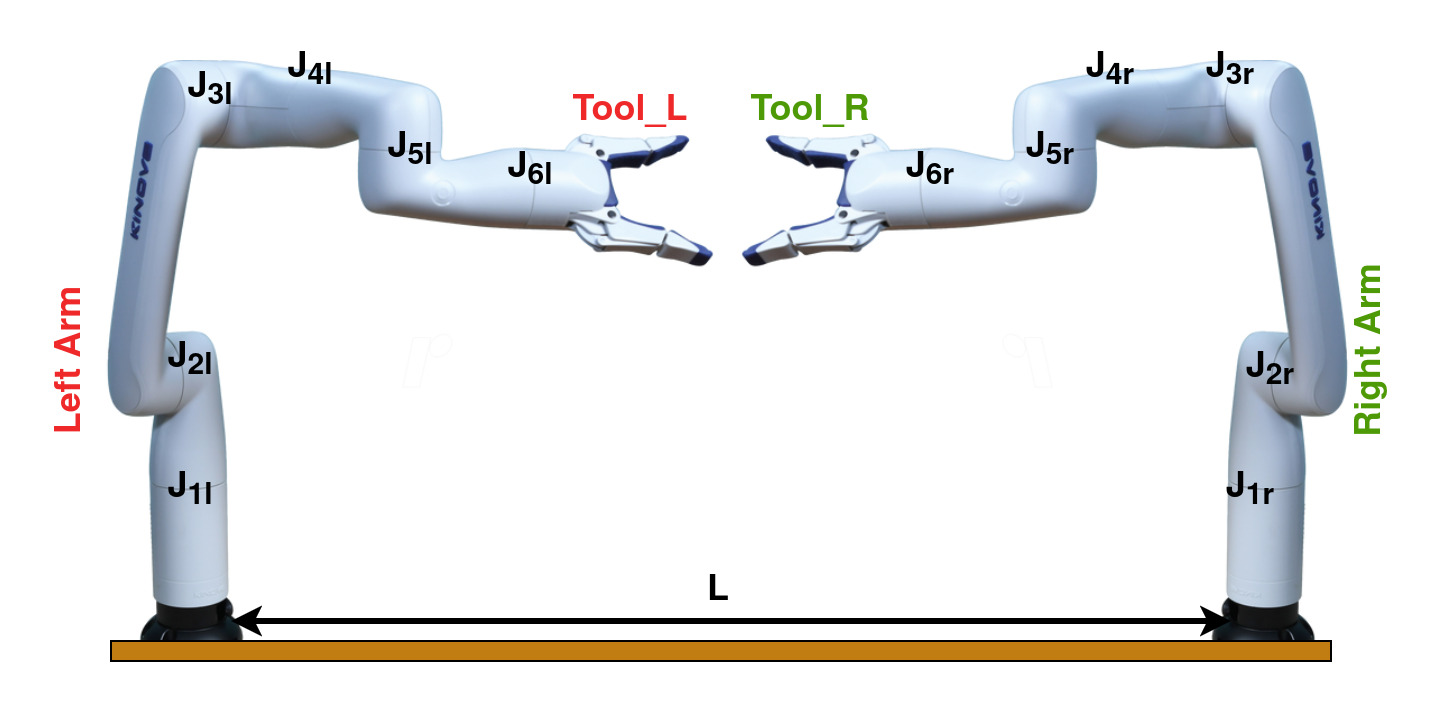
\includegraphics[width=1\linewidth]{Fig_1.jpg}
    \caption{Dual-Arm Setup for Distance calculation to avoid Inter-Arm Collisions.}
    \label{Dual-Arm}
\end{figure}
\begin{figure*}[htbp]
    \centering
    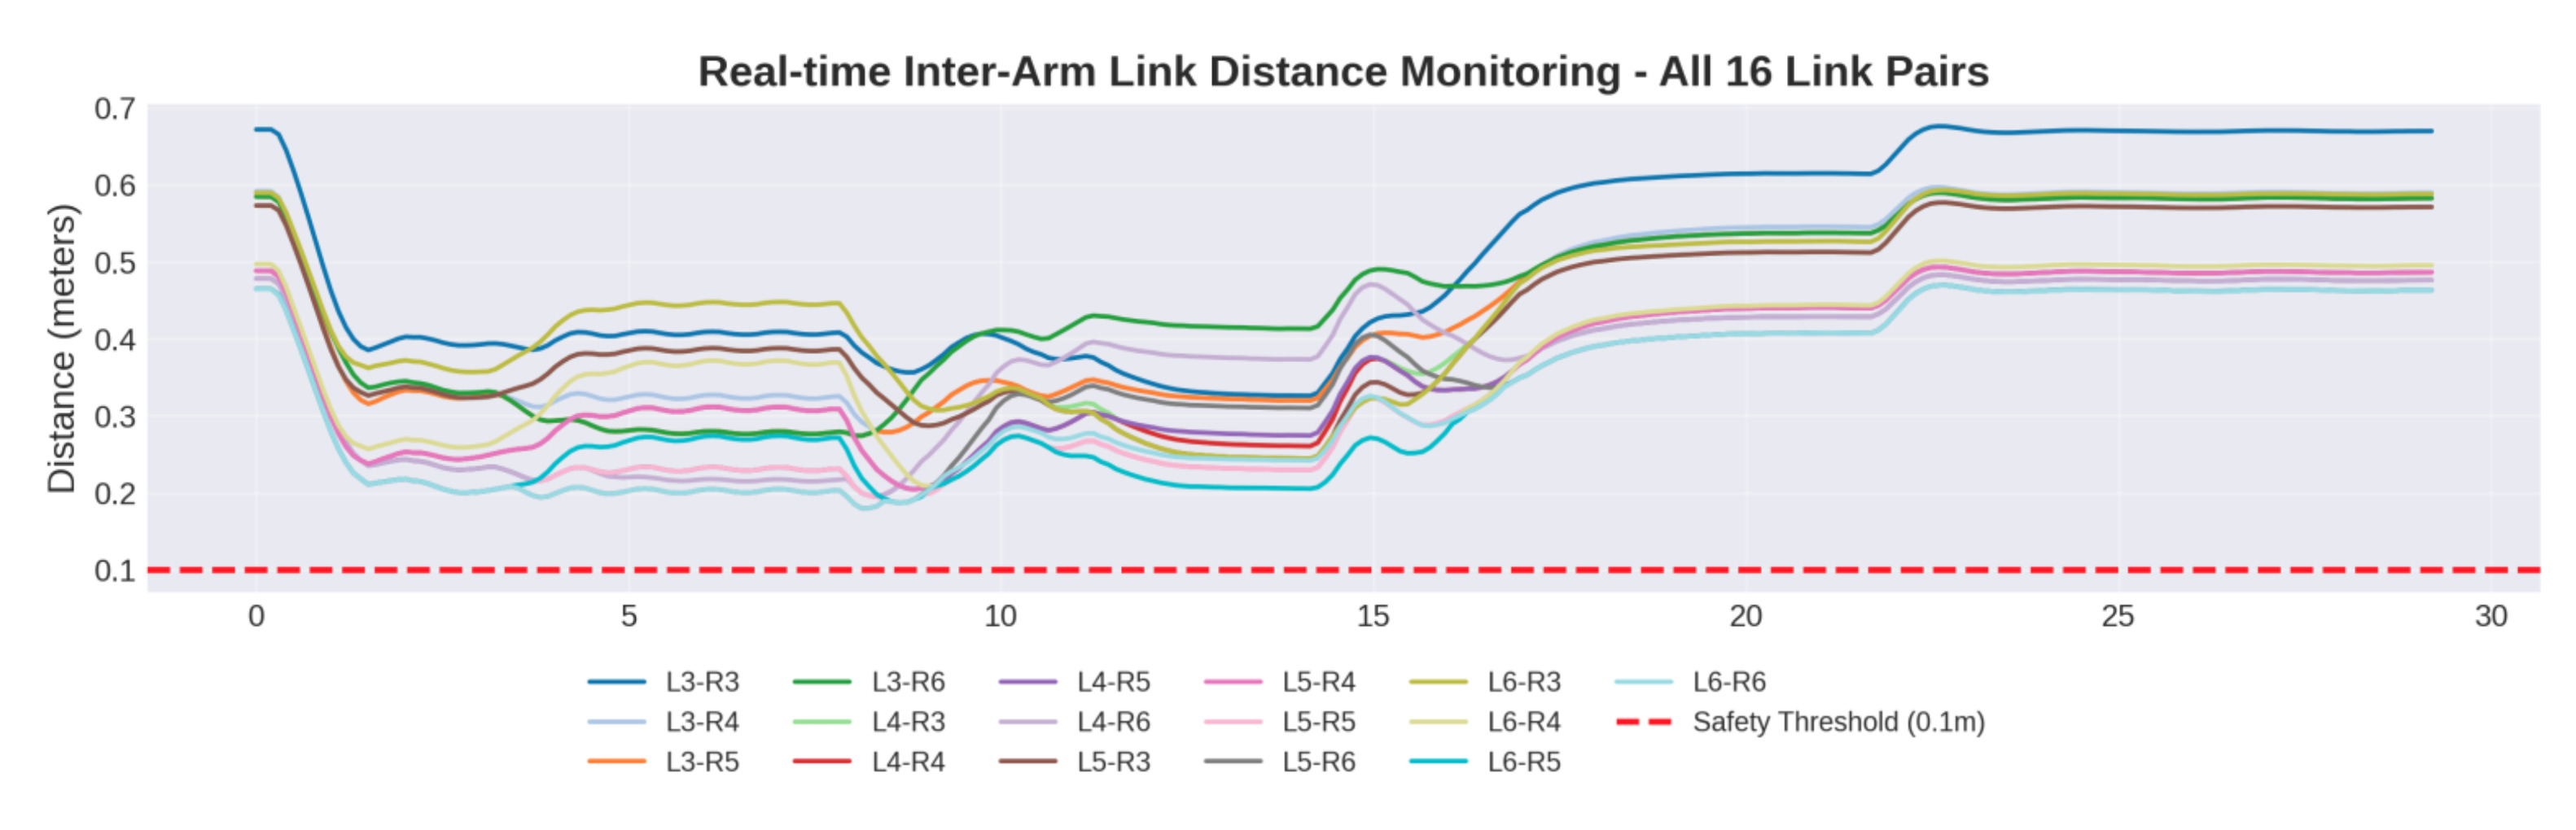
\includegraphics[width=0.8\textwidth]{Fig_2.jpg}
    \caption{Computation of inter-arm link distances of dual-arm manipulator system in real-time.}
    \label{fig:conti-dist}
\end{figure*}
\begin{equation}
    T_{B_{L}}^{B_{R}} =
    \begin{bmatrix}
    R_{lr} & p_{lr} \\
    0 & 1
    \end{bmatrix}
\label{transform_eq}
\end{equation}
\quad \text{(Right arm relative to left arm)}
\begin{equation}
    D_{inter} \in \mathbf{R}^{6 \times 6} : \quad D_{inter}[i,j] = d(L_l^i, L_r^j)
    \label{inter-arm}
\end{equation}
In practical implementation due to the base separation of two manipulators, the first two links of the dual-arm system never involve in collision during real-time table operations, distance matrix in Eq. \ref{inter-arm} can be reduced to $D_{inter} \in \mathbf{R}^{4 \times 4}$.
\begin{algorithm}
\caption{Multi-Arm Collision Distance Computation}
\begin{algorithmic}[1]
\REQUIRE Joint configurations $\{\theta_1, \theta_2, \ldots, \theta_n\}$
\ENSURE Minimum distance between any pair of segments from different arms

\FOR{each arm $i$}
    \STATE Compute $p_i^j = T_W^{B_i} \cdot T_{B_i}^{J_j^i} \cdot [0, 0, 0, 1]^T$
\ENDFOR

\STATE Initialize $D_{\text{inter}} \in \mathbf{R}^{6 \times 6}$

\FOR{each segment pair $(L_i^j, L_k^\ell)$ where $i \ne k$}
    \STATE Classify geometric configuration: Parallel / Intersecting / Skew
    \STATE Compute $d(L_i^j, L_k^\ell)$ using appropriate algorithm
    \STATE Store $d(L_i^j, L_k^\ell)$ in $D_{\text{inter}}[i,j]$
\ENDFOR

\RETURN $\min(D_{\text{inter}})$
\end{algorithmic}
\end{algorithm}

\begin{figure}[h!]
    \centering
    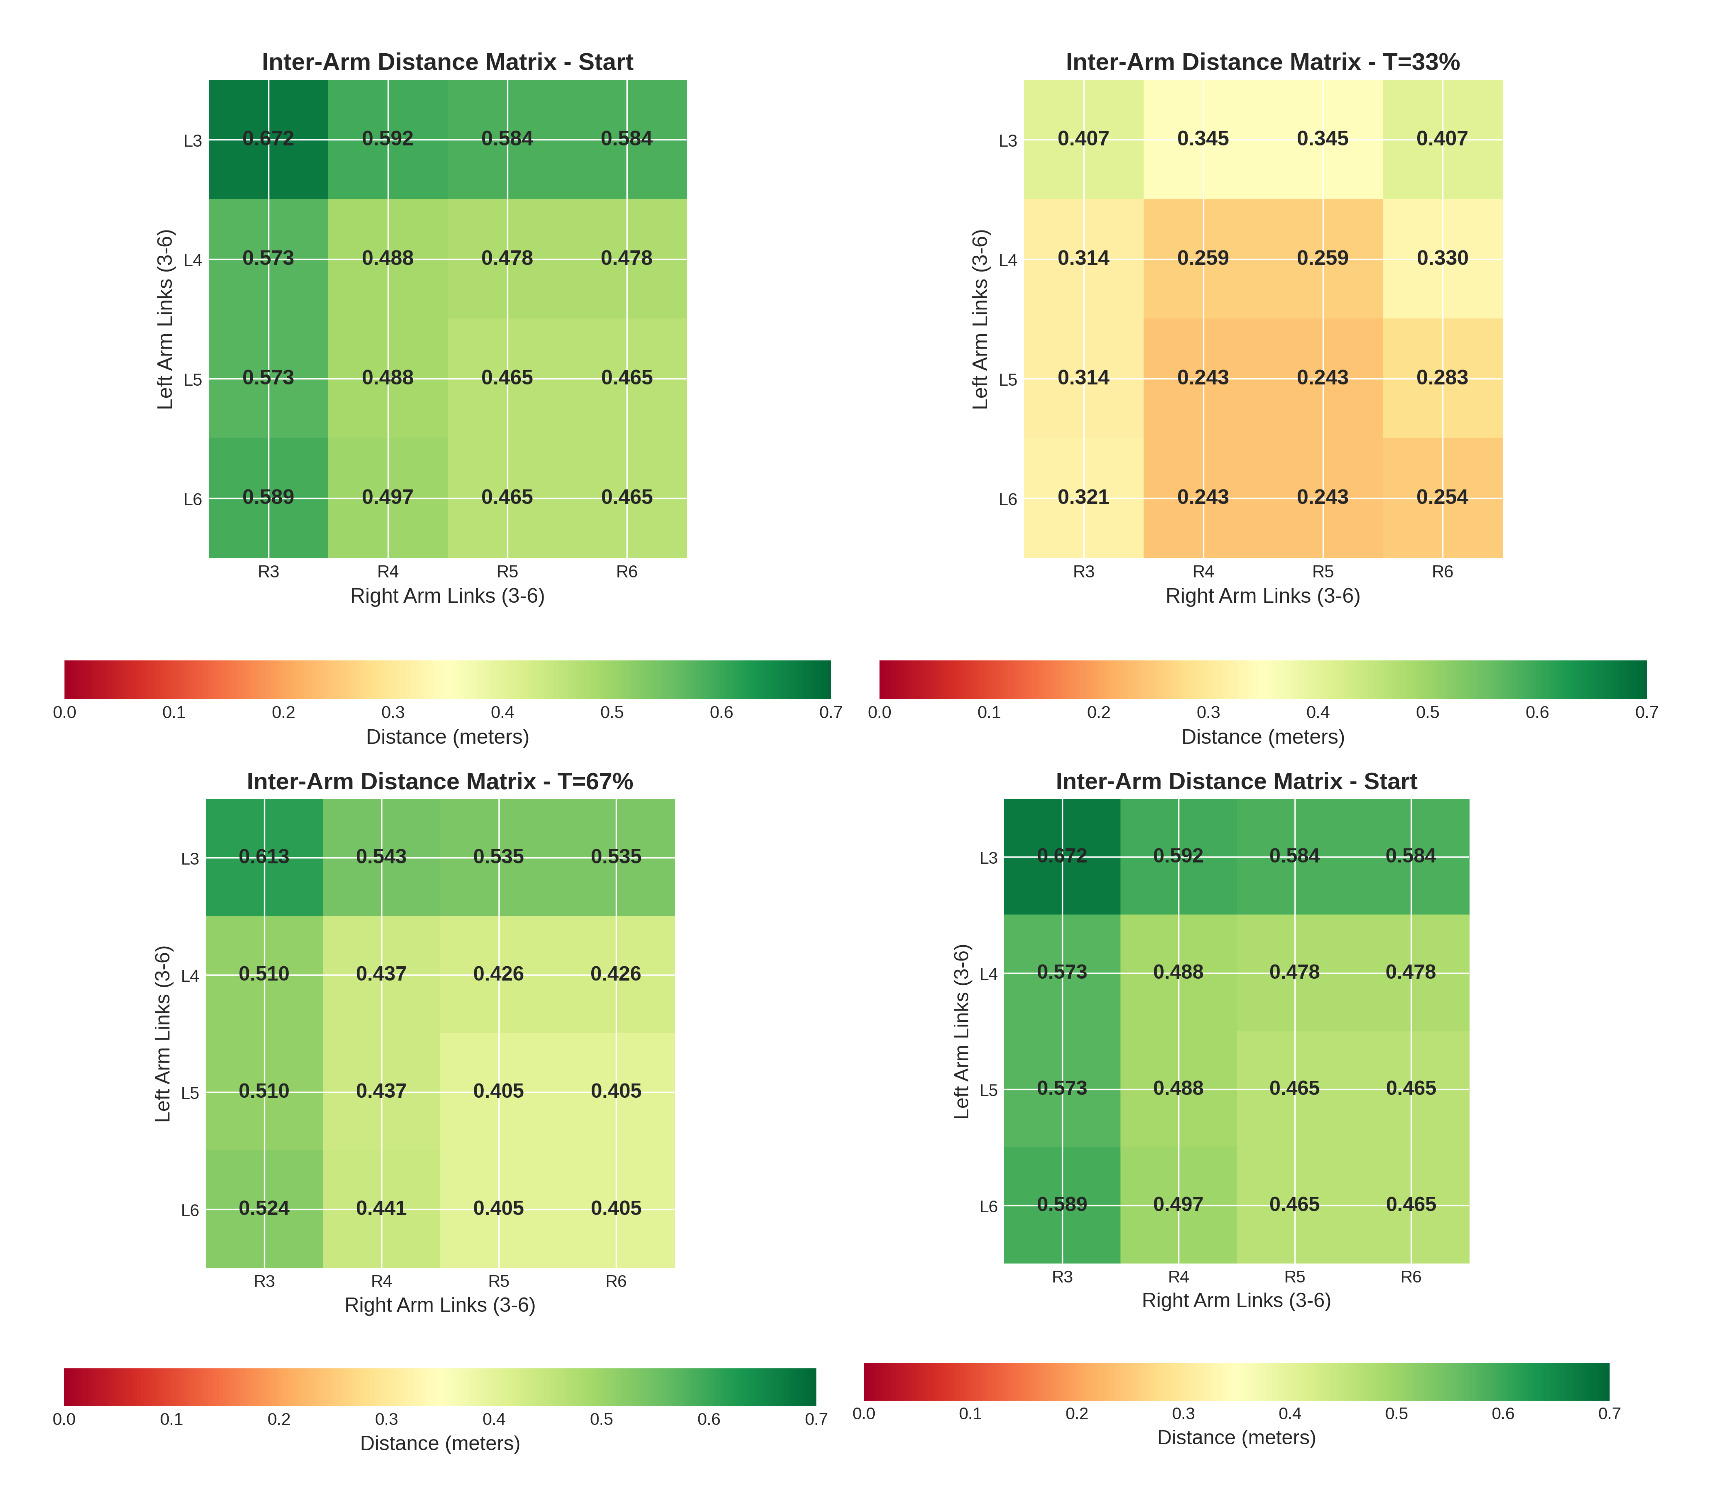
\includegraphics[width=\linewidth]{Fig_3.jpg}
    \caption{Collision distance Heatmap start from safe position, both arms approached each other(intense in heatmap), move far, again reached to safe positions.}
    \label{fig:coll-heat}
\end{figure}
\begin{figure}[h!]
    \centering
    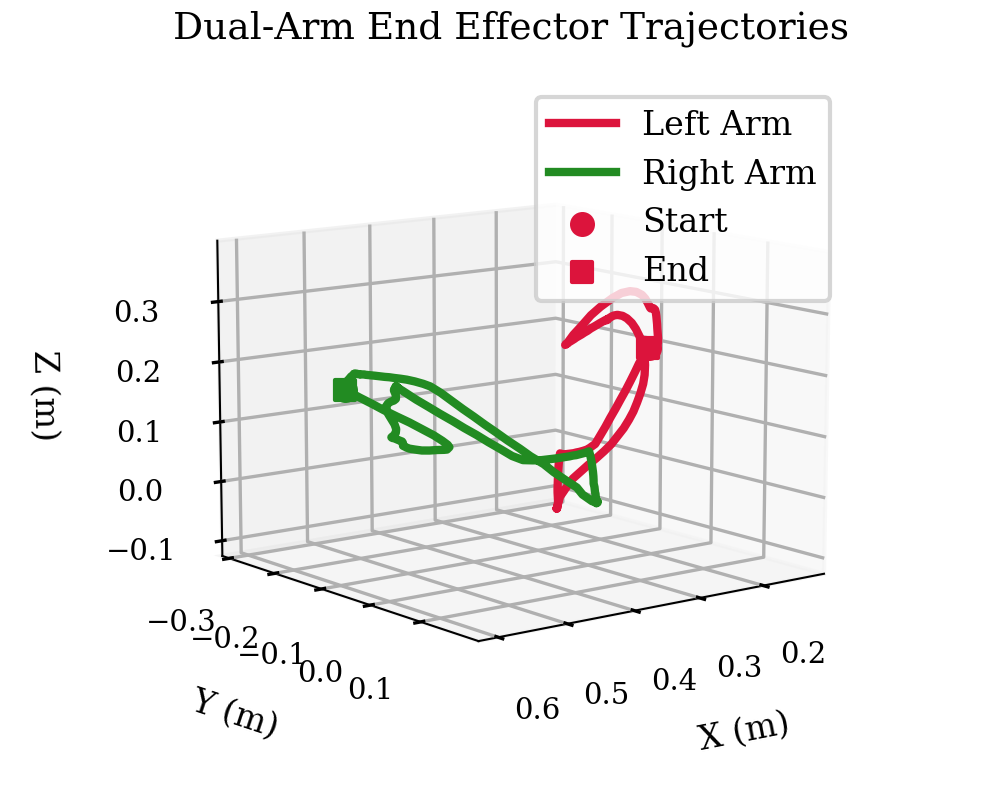
\includegraphics[width=1\linewidth]{Fig_4.png}
    \caption{Trajectory tracking to illustrate the real-time distance computation for multi-arm manipulator system(dual-arm)}
    \label{fig:dual-trajec}
\end{figure}
\section{Experiment and Results}
\label{results}
For validation of our proposed methodology, an experimental setup as shown in Fig.\ref{Dual-Arm} of two Kinova Gen3 Lite 6 DOF manipulators with non-spherical wrist structure are employed. The manipulators are table-mounted and arranged facing each other to represent bi-manual manipulation scenarios. Both manipulators are connected to a PC (Intel NUC9, 32 GB RAM, RTX3060 12GB) through Ethernet connections. The Kinova manipulators are accessed using TCP/IP connections and controlled using the Kinova-Kortex API \cite{Kinovarobotics}.

The dual-arm system is controlled through end-effector velocity commands (twist control), targeting positions of [0.385, 0.045, -0.01] m for the left arm and [0.327, 0.050, -0.01] m for the right arm during the pick phase. Continuous real-time inter-arm distance calculations for all 16 link pairs (L3-L6 to R3-R6) are presented in Fig.~\ref{fig:conti-dist}, with an arbitrary safety threshold reference of 0.1 m.
The distance evolution is visualized through heatmaps in Fig.~\ref{fig:coll-heat}, showing four critical phases: initial separation (Start), approach phase (T=33\%), closest proximity during pick operations (T=67\%), and final separation (End). The color intensity variations clearly demonstrate distance changes - darker regions indicate closer proximity between link pairs, with minimum distances of approximately 0.2 m observed during the pick phase. Critical link pairs L4-R4 and L5-R4 show the closest approach, dropping to 0.243 m and 0.259 m respectively at T=33\%. The computed distance matrix was successfully integrated with traditional artificial potential field methods to demonstrate collision avoidance during coordinated dual-arm manipulation tasks. The complete dual-arm end-effector trajectories are shown in Fig.~\ref{fig:dual-trajec}, illustrating the coordinated motion from home positions through pick, place, and return phases. The continuous distance monitoring demonstrates the system's capability to track inter-arm proximity in real-time, providing the foundational data necessary for implementing collision avoidance strategies. Experimental results of the proposed methodology are available in the repository \cite{git_repo}.

\section{Conclusion and Future scope}
\label{conclusion}
This paper presents a comprehensive mathematical framework for real-time distance monitoring in table-mounted multi-arm manipulator systems. The kinematics-based approach eliminates dependency on external sensors while providing continuous inter-arm distance calculations through forward kinematics and line segment modeling. The practical implementation of the proposed methodology on dual-arm manipulators demonstrates practical applicability for distance monitoring. The computed distances integrated with collision avoidance techniques like traditional APF methods validate the practical applicability of the proposed method.

In our future work, we will work to overcome the present assumption that the shared workspace is free from external obstacles and the practical validation limited to dual-arm systems. Future work will extend the framework to multi-arm systems (n>2) with variable DOF manipulators. Additionally, we will advance collision avoidance techniques using the current real-time distances for complex coordinated motions for multi-arm systems to meet industrial automation requirements.
\bibliographystyle{ieeetr}
\bibliography{ref_iccas}
\end{document}